\documentclass[12pt]{article}
\usepackage{graphicx}
\usepackage[utf8]{inputenc}
\graphicspath{{../plots/}}


\title{Cancellation Rates Model}
\author{Morgan Bruce}
\begin{document}

\maketitle

\section*{Problem}
Over recent quarters, our hotel chain has been experiencing an increased booking cancellation rate. This results in lost revenue from empty rooms that are not filled due to being associated with previous reservations.

\section*{Solution}
Our team investigated the data of the hotel bookings to both find patterns that could indicate reasons for increased cancellations, and developed a model that could help with predicting if a customer is likely to cancel a booking, so that we can act proactively to fill the empty room to prevent lost revenue.

\section*{Results}
The investigation of the dataset did back-up the hypothesis that cancellation rates were increasing. Figure 1 shows the rate of cancellations, separated by the hotel.

\begin{figure}
    \centering
    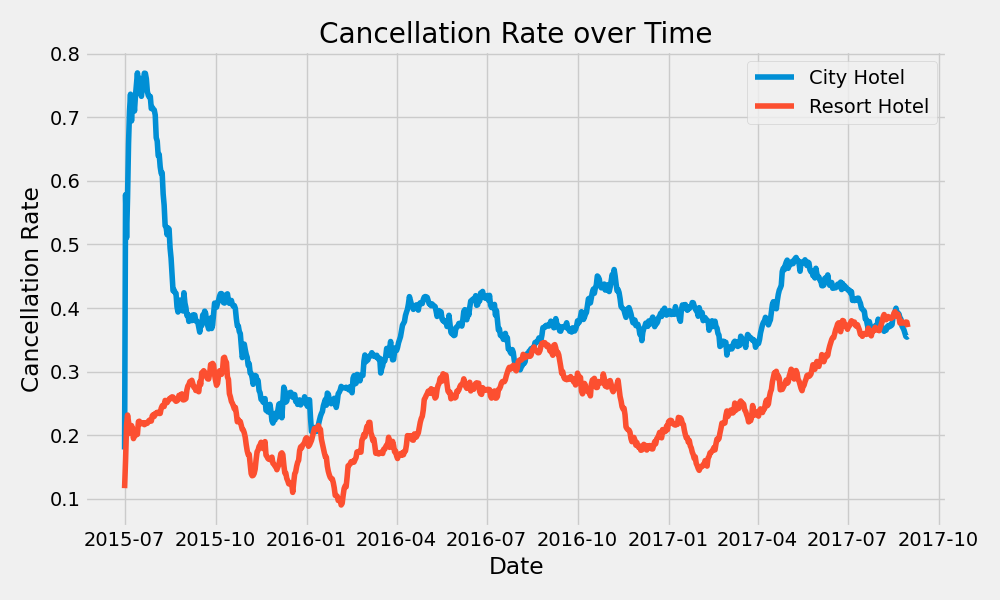
\includegraphics[scale=0.5]{cancel_rate_over_time.png}
    \caption{Cancellation rates over time}
\end{figure}

The dataset of bookings is complex, and does not yield an obvious answer to the reason for the increased cancellations. There are some potential indicators, such as customers with repeated cancellations being more likely to cancel in the future, or certain agencies having abnormally high rates of cancellation, which possibly comprises the majority of the increase in cancellations.

Our team also developed a classification model to predict if a customer is likely to cancel their booking. We held the most recent quarter of bookings separate, and trained the model on the previous historical data before testing its performance on the most recent quarter. In this fashion, our XGBoost classification model achieved an accuracy of over 80\% on test data in classifying if a booking will cancel or not, as shown in Figure 2.

Our team envisions that this model could be used to remain proactive against lost revenue due to bookings. In particular, customer service could reach out to bookings that have a high likelihood of cancelling, to ensure that all needs are being met by the customer. Additionally, similar to how airlines will overbook planes with the expectation of some customers not showing up, bookings predicted to be cancelled could be overbooked with the expectation that the customer is likely to cancel anyways.

Due to the test scheme of holding out the most recent quarter of data, our team is confident that if this model is put into production, it will perform consistent to testing.

\begin{figure}
    \centering
    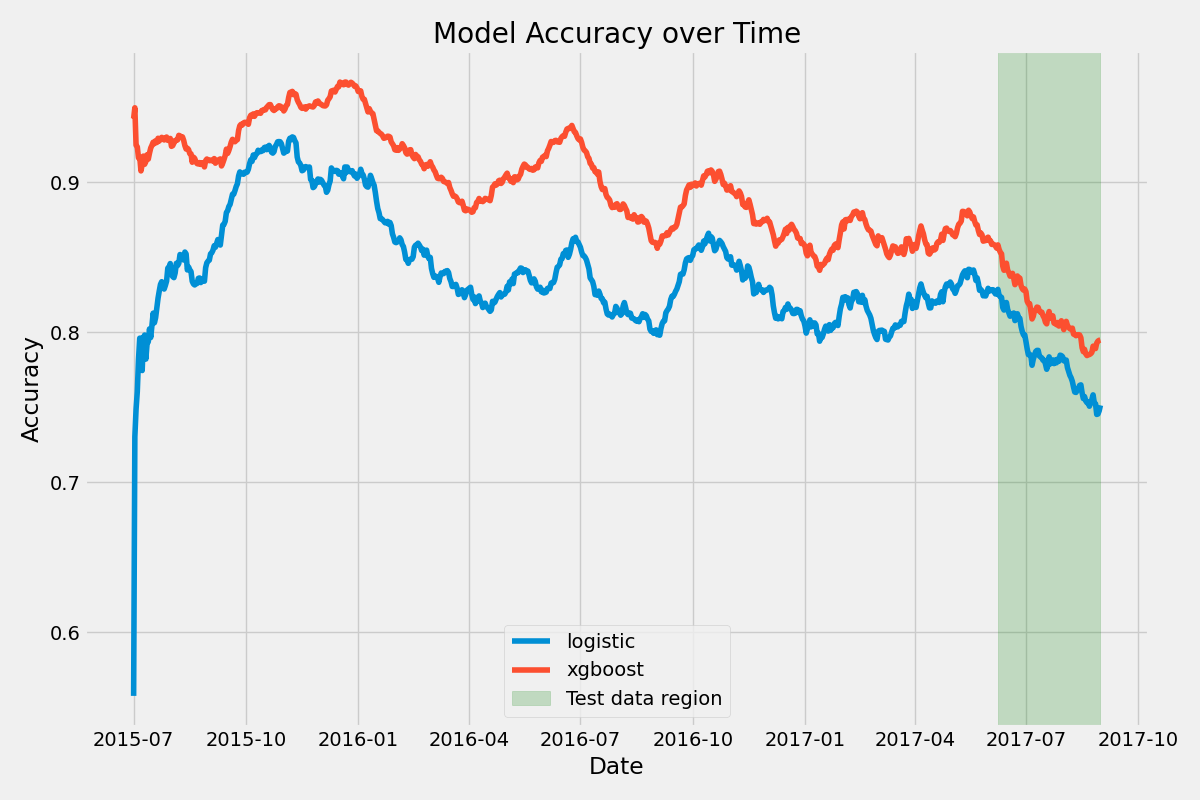
\includegraphics[scale=0.45]{model_accuracy.png}
    \caption{Plot of two version of our model over the dataset, averaged over 4 weeks time.}
\end{figure}

\end{document}